\section{The Necron Tombworlds}


\subsection{Building a Necron Army}

In games of the Horus Heresy: Age of Darkness, the models under a given player’s control are referred to as that player’s army. Each army is composed of a single Force Organisation chart (most commonly using the Crusade Force Organisation chart), which will include one or more Detachments. An army whose Primary Detachment is selected from any Army List is considered to have the Faction of that Primary Detachment (for example, an army whose Primary Detachment was selected from the Necrons List would be considered an Necron army). Units from various Sub-factions cannot be mixed in the same Detachment, unless a Special Rule or other ability permits this.

Other, non-Primary, Detachments in the same army may be selected from any other Army List - following any additional restrictions applied, such as the ones on the next page - but each Detachment may only include units from a single Army List, unless another Special Rule states otherwise.

When selecting a Primary Detachment, you must also choose a Sub-Faction for that detachment, in the form of a Necron Dynasty. Each Dynasty provides special bonuses and options for their units and determines the Alliance Levels between other Sub-Factions.

In addition, each Dynasty has a number of allied units that are usually attached to its Tomb Worlds, whether that be Triarch Praetorians watching over the slumbering necrons, a Destroyer Cult filling part of their ranks, or Flayed Ones lurking at the fringes. As such, a Primary Detachment is also allowed to incorporate a number of Allied Units without requiring an entire Allied Detachment be taken, so long as the number of points spent on Triarch, Destroyer, and Flayed models does not exceed 25\% of the army's total points.

\newpage
\subsection{Force Organisation Charts and Detachments}

\newpage
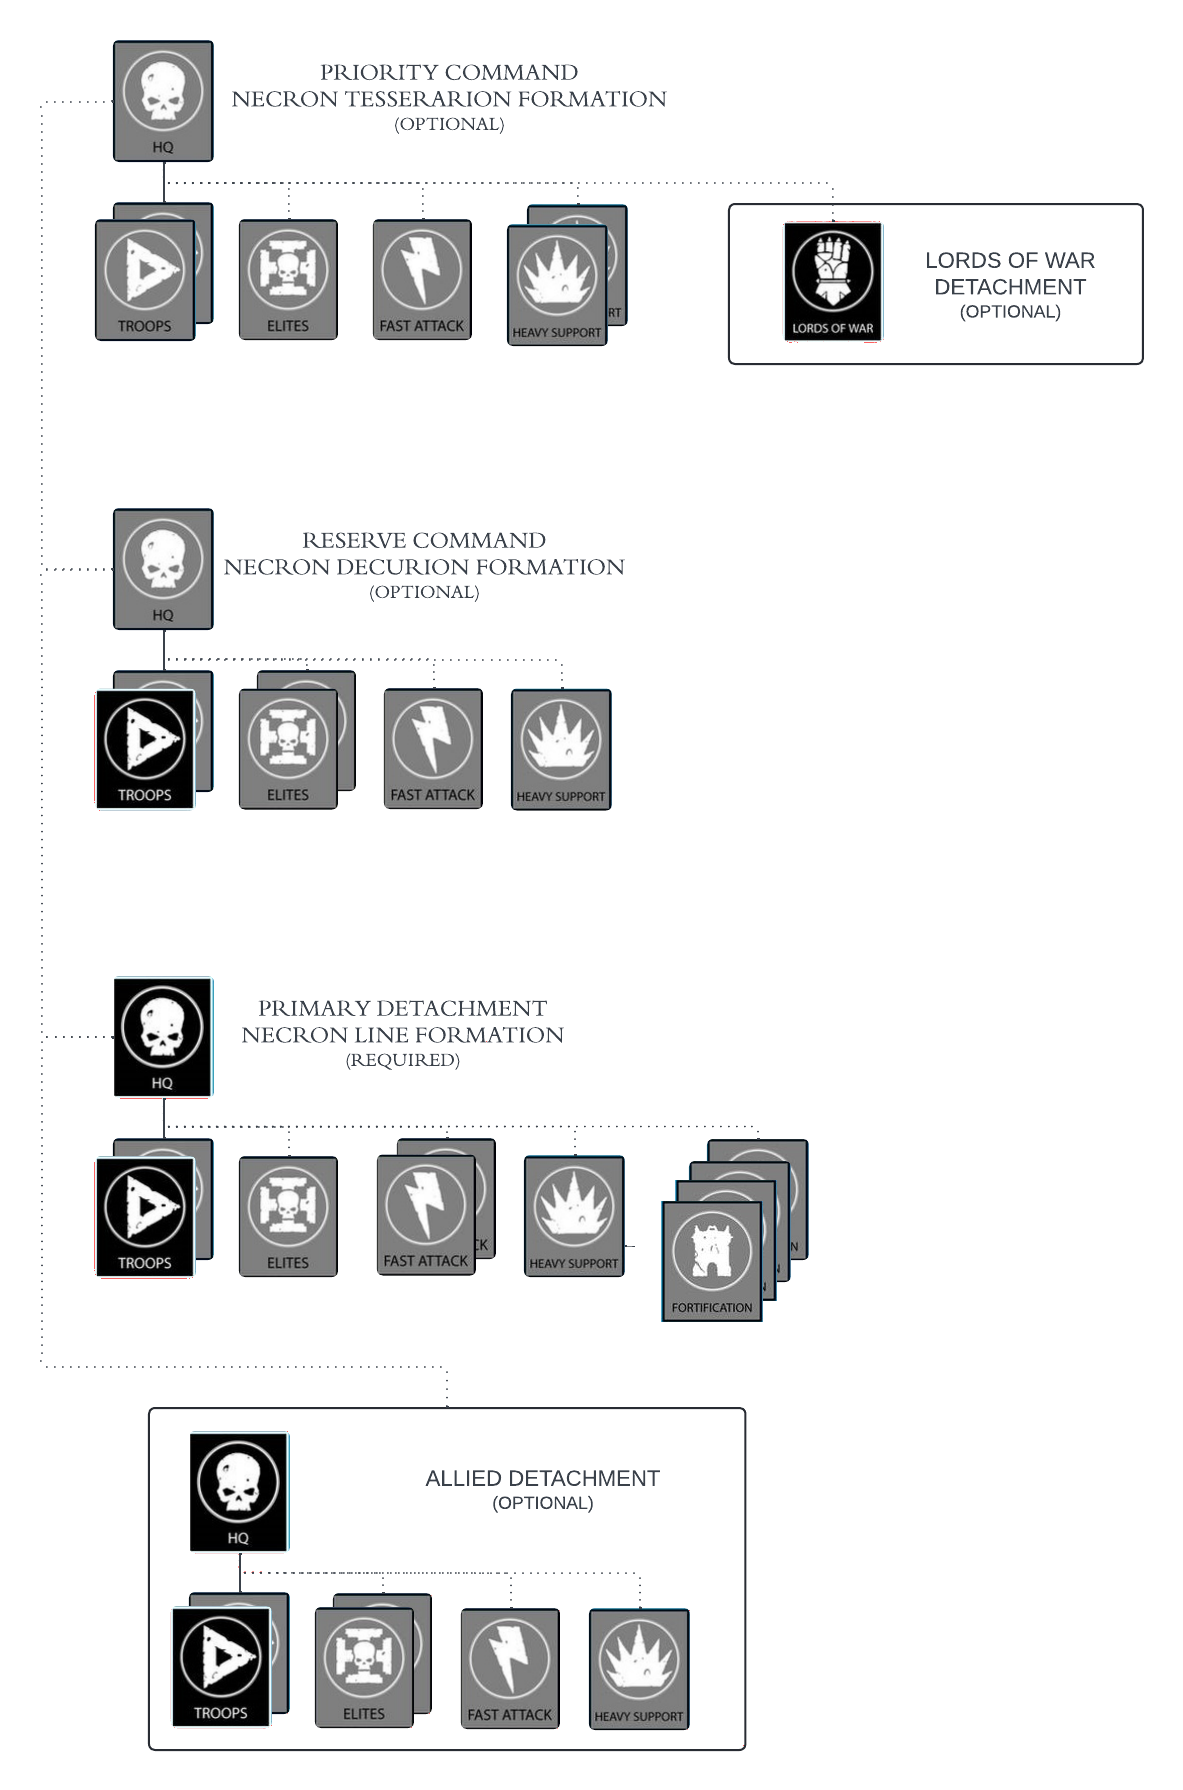
\includegraphics[width=500pt, height=750pt]{Org chart.png}

\newpage
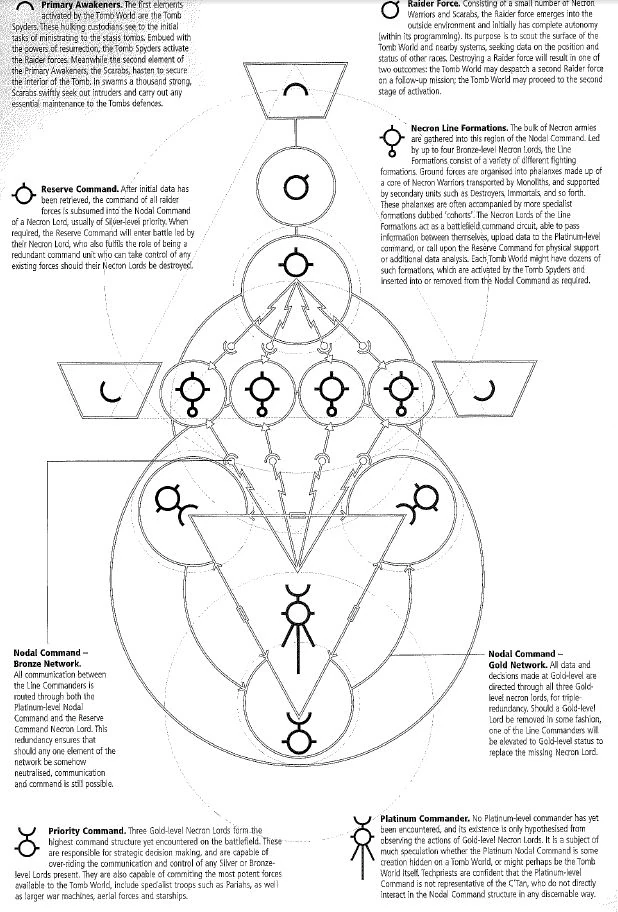
\includegraphics[width=500pt, height=750pt]{nodal.png}